\section{Rakenduse funktsionaalsus ja vaated}
Järgnevalt kirjeldatakse töö tulemusena valminud rakenduse funktsionaalsust ning analüüsitakse, kuidas see täidab töö alguses püstitatud kasutusjuhte. Iga kasutusjuhi juurde on lisatud kuvatõmmis, et visualiseerida, kuidas rakendus toimib.

\subsection{Rakenduse kasutajaliidese tutvustus}
All joonisel on näha rakenduse põhivaade, millel on märgitud selle põhisektsioonid:
Kontrollpaneel: see on rakenduse menüü, kus kasutajal on võimalik: salvestusi hallata, valida visualiseerimise tegevus (1. tunnuste visualiseerimine või 2. sarnasuse visualiseerimine), peale tulemuste visualiseerimist andmeid eksportida.
Helisalvestuste esitaja (Recording Player): võimaldab helifaili mängimist ning kuvab selle amplituudi visualisatsiooni.
Visualiseerimise vaade (Visualisation View): vaates kuvatakse kontrollpaneelis tehtud valikute põhjal genereeritud jooniseid.
4.	Tabelvaade (Table View): vaates kuvatakse visualisatsiooni andmed tabeli kujul.

\begin{figure}[H]
    \centering
    \includegraphics[width=\textwidth]{figures/rakenduse-põhivaate-osad.png}
    \caption{\textit{Rakenduse põhivaade ja selle osad}}
    \label{fig:rakenduse-põhivaate-osad}
\end{figure}

\subsection{Kasutusjuhtude analüüs}
All kirjeldatakse, kuidas loodud rakendus täidab igat funktsionaalsete nõuete kasutusjuhtu.

\textbf{Salvestuste töötlemine ja haldamine
}

Kasutusjuhud nõuetes:
\begin{itemize}
    \item GeMAPS tunnuste eraldamine kõnefailidest
    \item Salvestuste töödeldud andmete kustutamine
\end{itemize}

Realiseerimine rakenduses: Kontrollpaneelis asuv nupp \textit{Manage Recordings} avab salvestuste haldamise akna. Kasutaja saab \textit{Import Files} nupu abil valida \texttt{.wav} ja \texttt{.TextGrid} faile, mille järel OpenSMILE’i abil eraldatakse GeMAPS tunnused ja salvestatakse MongoDB andmebaasi. Joonis !! illustreerib salvestuste halduse akent, kus on näha töödeldud salvestuste nimekiri.
Tulemus: Kasutaja saab töödelda ja hallata salvestusi. Rakendus kuvab nii õnnestumise- kui ka veateateid (kuvatõmmised lisa 2)
\begin{figure}[H]
    \centering
    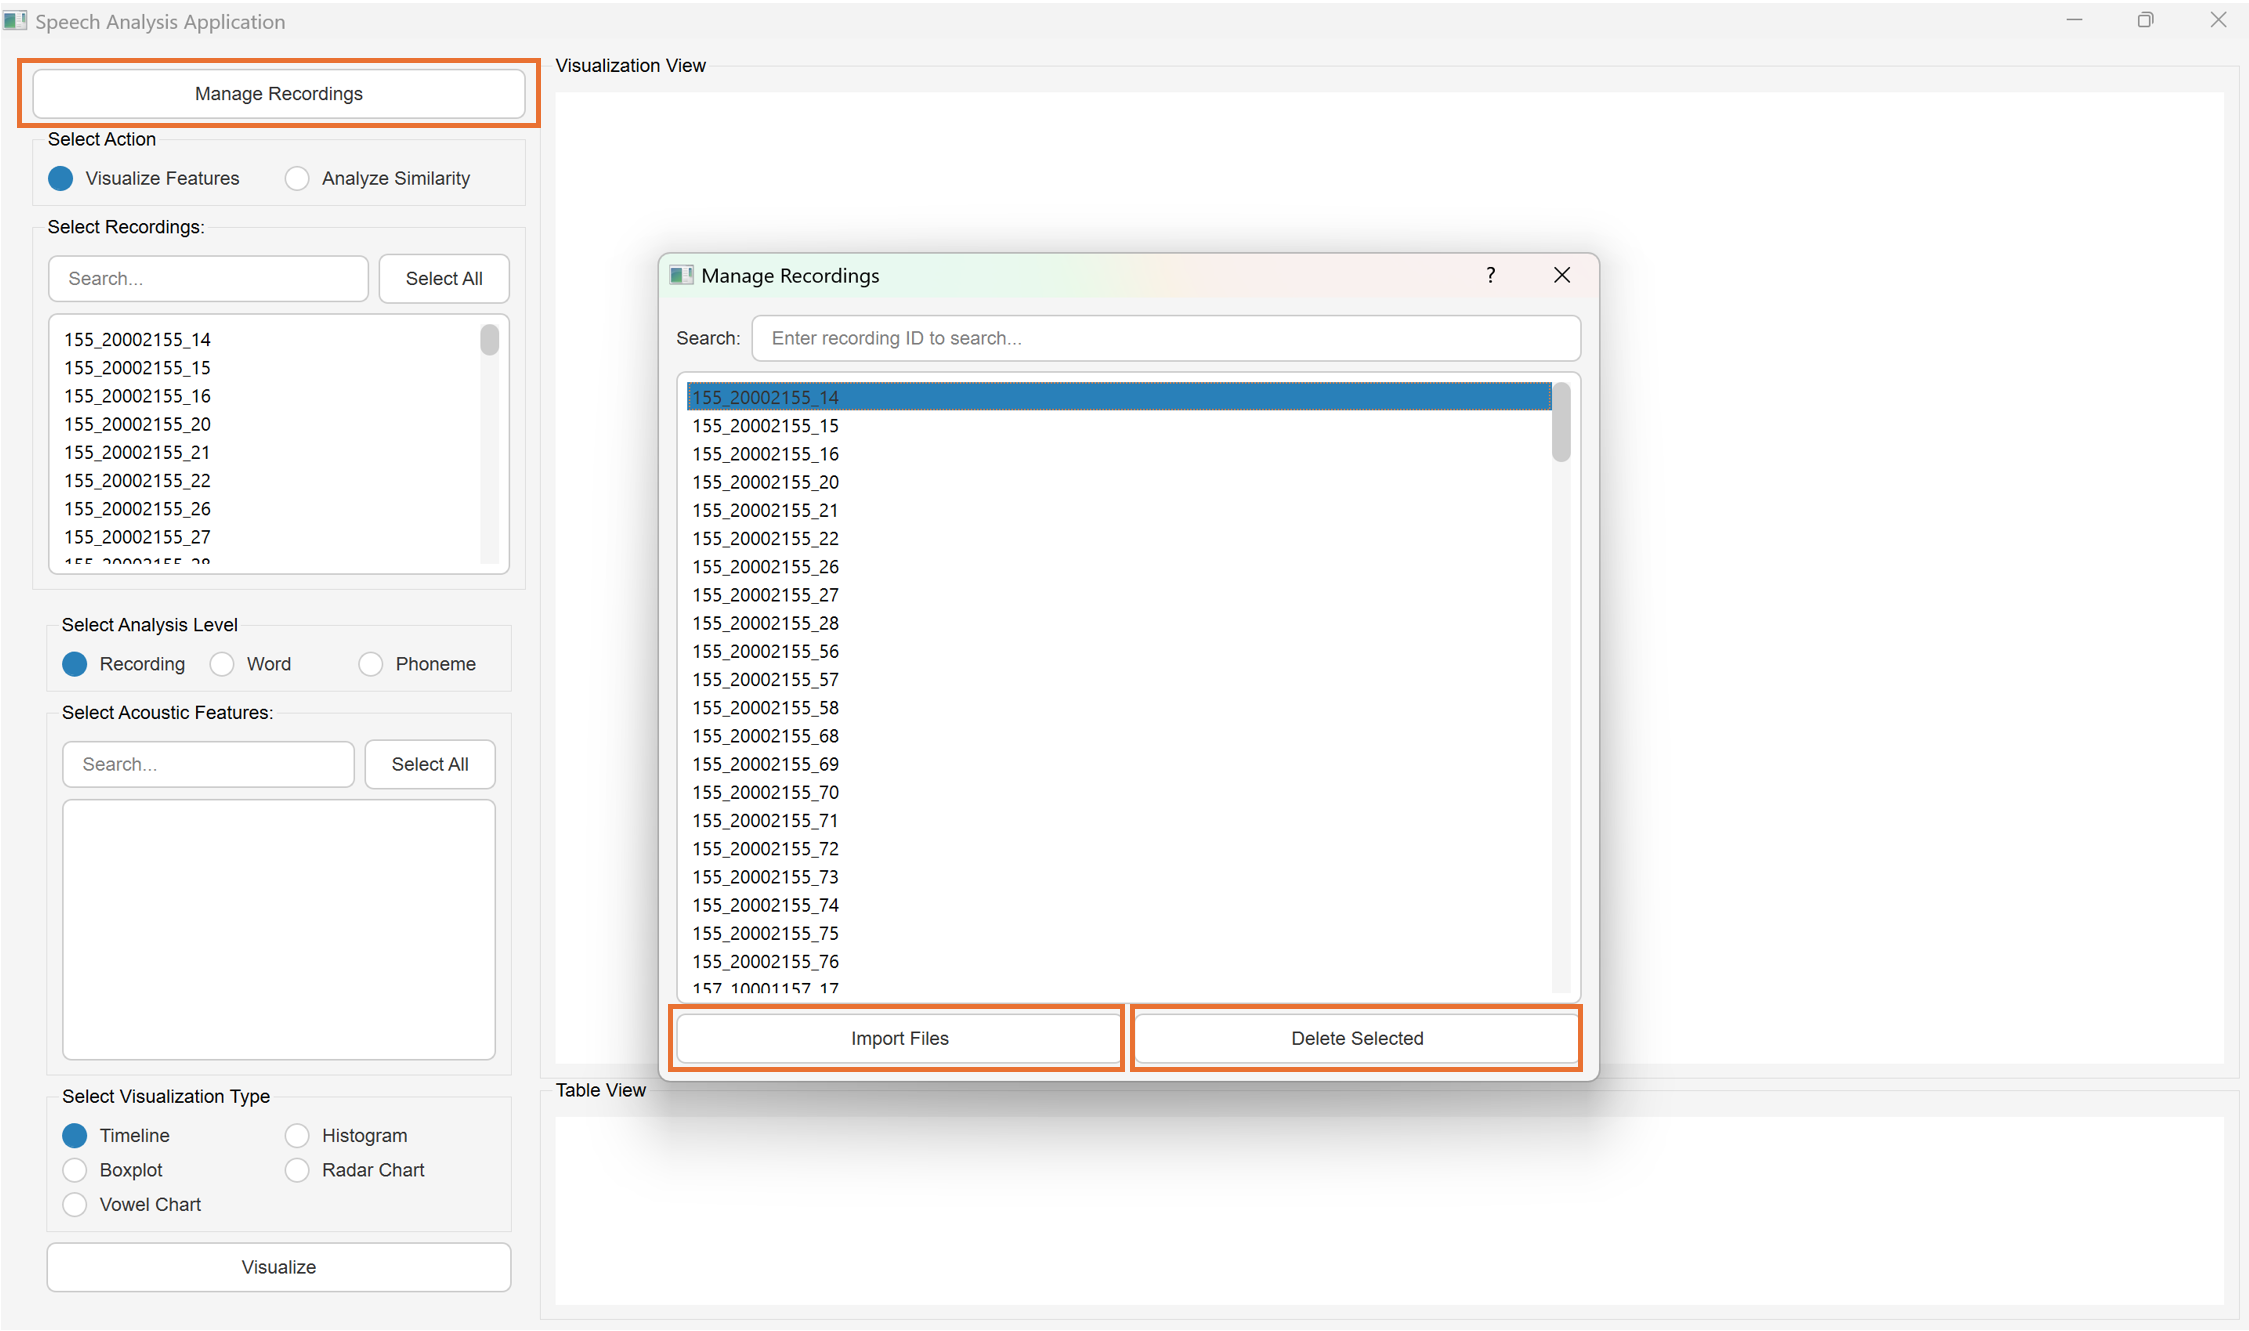
\includegraphics[width=\textwidth]{figures/rakenduse-salvestuste-haldus.png}
    \caption{\textit{Rakenduse salvestuste haldus}}
    \label{fig:rakenduse-salvestuste-haldus}
\end{figure}

\textbf{Tunnuste visualiseerimine
}

Kasutusjuht nõuetes: Tunnnuste visualiseerimine
Realiseerimine rakenduses:
\begin{enumerate}
    \item Kasutaja valib Visualize Features.
    \item Valib salvestuse(d) (Select Recordings).
    \item Määrab, kas soovitakse vaadata tunnuseid salvestuse, sõna või foneemi tasandil (Select Analysis Level).
    \item Kui valiti foneemi või sõna tasand, tuleb valida ka sõnad või foneemid.
    \item Valida konkreetsed GeMAPS tunnused (Select Acoustic Features).
    \item Valida sobiva graafikutüübi (nt ajatelg, karp-, histogramm, radar, vokaalikaart).
    \item Pärast nupule Visualize klõpsamist kuvatakse Visualization View, kus on: Interaktiivne graafik, mille paremas ülanurgas tööriistad (suurendus, pildi eksport, jms). Tabelvaade (Table View) samas aknas, et vaadata punktandmeid tabelina.
\end{enumerate}

\begin{figure}[H]
    \centering
    \includegraphics[width=\textwidth]{figures/rakenduse-tunnus-sõna-timeline.png}
    \caption{\textit{Joondiagrammi näide ühe sõna ja tunnuse visualiseerimisel}}
    \label{fig:rakenduse-tunnus-sõna-timeline.png}
\end{figure}

\textbf{Sarnasuse analüüs
}

Kasutusjuht: Sarnase kõneleja leidmine

Realiseerimine rakenduses
\begin{enumerate}
    \item Kasutaja valib Analyze Similarity.
    \item Kasutaja määrab salvestused, mida omavahel võrrelda (Select Recordings).
    \item Valib ühe Target Recording, millega teisi võrrelda.
    \item Sisestab hulga, mitu sarnaseimat salvestust soovitakse saada (Number of Similar Items).
    \item Valib meetodi: Cluster Analysis (PCA + KMeans), Feature Similarity Bars (koosinussarnasus) või PCA-Based Similarity Bars (koosinussarnasus PCA ruumis).
    \item Pärast nupuvajutust arvutab rakendus statistika (nt klasterdamise või koosinussarnasuse), seejärel kuvatakse Visualisation View, kus on: tulpdiagramm, mis näitab salvestuste sarnasuse väärtust,
    või hajuvusdiagramm (klastrite korral), mis eristab klastreid värvidega ning märgib sihtsalvestuse ja kõige sarnasemad salvestused eraldi sümbolitega.
\end{enumerate}
\begin{figure}[ht]
    \centering
    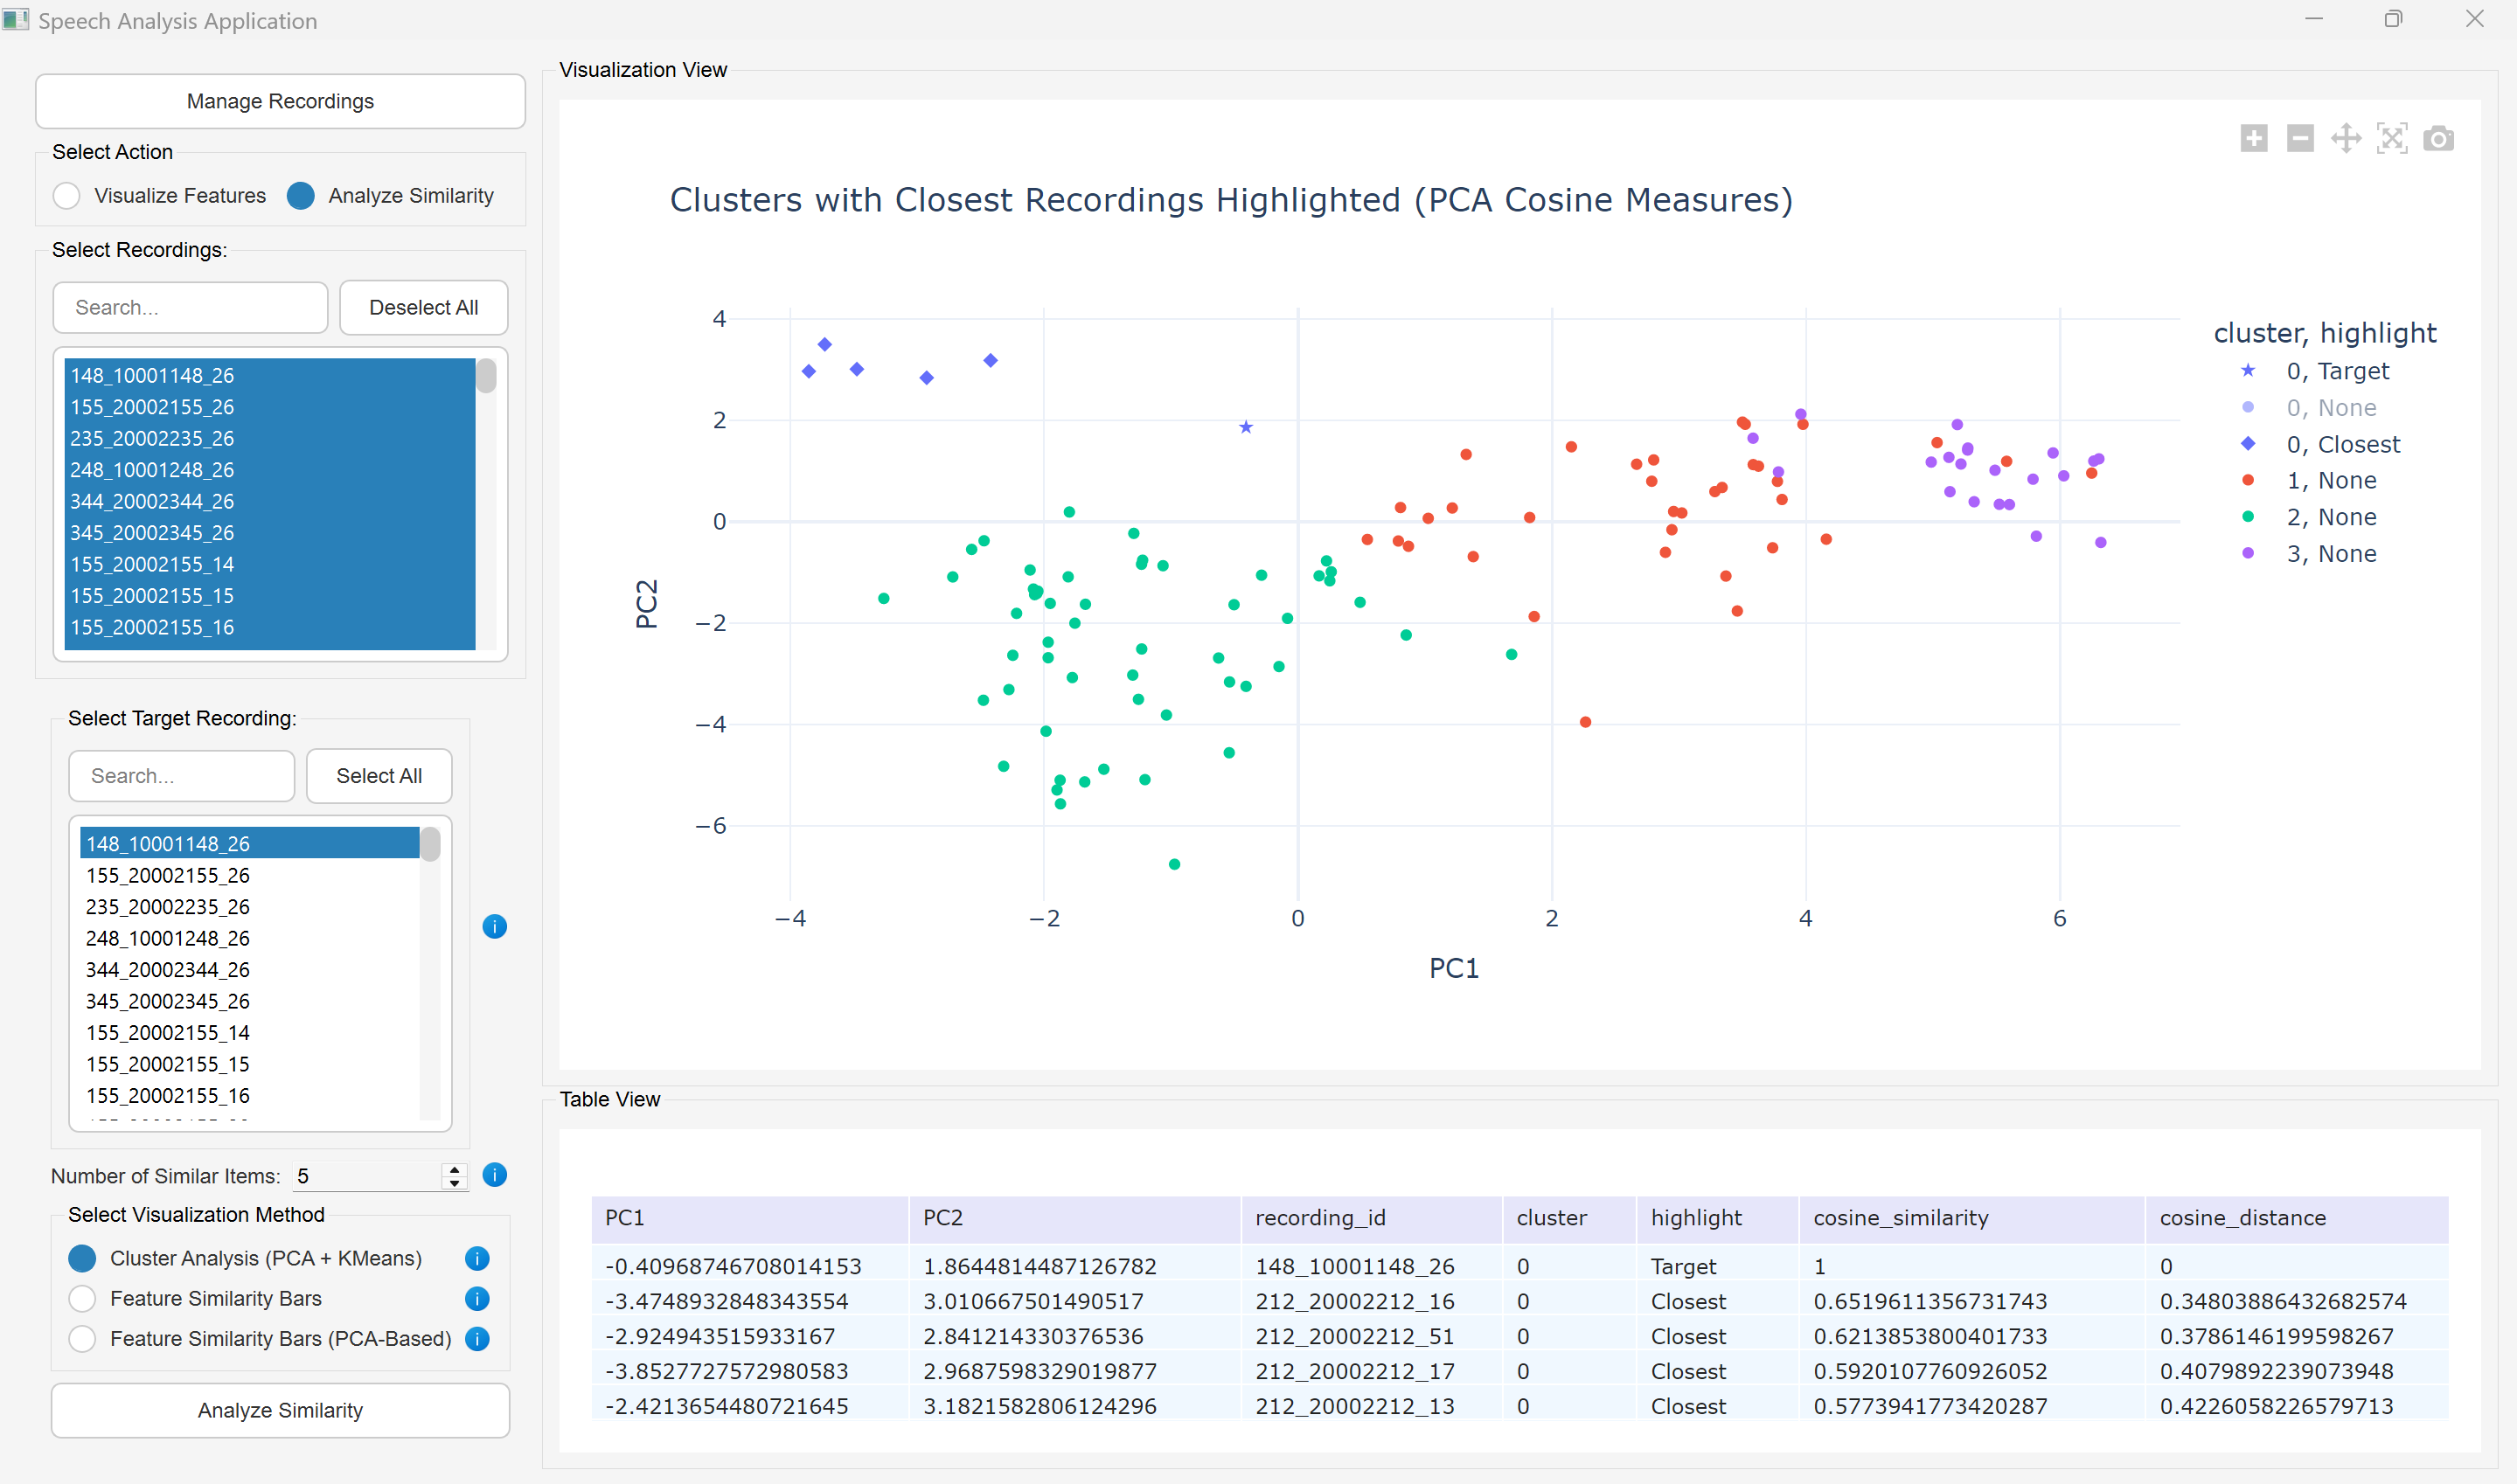
\includegraphics[width=\textwidth]{figures/rakenduse-sarnasus-cluster-closest.png}
    \caption{\textit{PCA koosinussarnasuse ja klastrite visualiseerimine hajuvusdiagrammil}}
    \label{fig:rakenduse-sarnasus-cluster-closest}
\end{figure}

\textbf{Helisalvestuse esitamine ja helilaine visualiseerimine
}

Kasutusjuht nõuetes: Helisalvestuse esitamine ja helilaine visualiseerimine

Realiseerimine rakenduses:
\begin{enumerate}
    \item Recording Player sektsioonis, kuvatakse rakenduse „data“ kaustas asuvad salvestused.
    \item Kasutaja valib faili ning vahutab \textit{Play} nuppu.
    \item Rakendus mängib helisalvestust, samal ajal kuvatakse helilaine
\end{enumerate}

\textbf{Andmete ja visualisatsioonide eksportimine}

Kasutusjuht nõuetes: Andmete ja visualisatsioonide eksportimine

Realiseerimine rakenduses
Iga valminud graafiku kohal on kaamera märgiga nupp (Plotly sisseehitatud funktsioon). See võimaldab kasutajal salvestada staatilise pildifaili.
Lisaks on kontrollpaneelis Export Graph Data (JSON) nupp, mis salvestab kasutatud andmed JSON-vormingus.

\section{Tulemuse võrdlus olemasolevate lahendustega}
Järgnevalt võrreldakse valminud rakenduse funktsionaalsust Kõneveebi Audiofailide akustiliste omaduste võrdlemise lahendusega. Kuna see tööriist on alternatiivsetest lahendusest kõige sarnasem oma fookuse, eesmärgi ja funktsionaalsuse poolest. Kuigi Praat või VoiceSauce on palju laiemalt kasutatud akustiliste tunnuste analüüsimisel, on nende fookus ja funktsionaalsus palju laiem ning nad ei keskendu kitsalt eGeMAPS-tunnuste komplektile, nagu Kõneveebi lahendus ja ka loodud rakendus. Seega on sobivam rakendust võrrelda Kõneveebi lahendusega.

\begin{figure}[H]
    \centering
    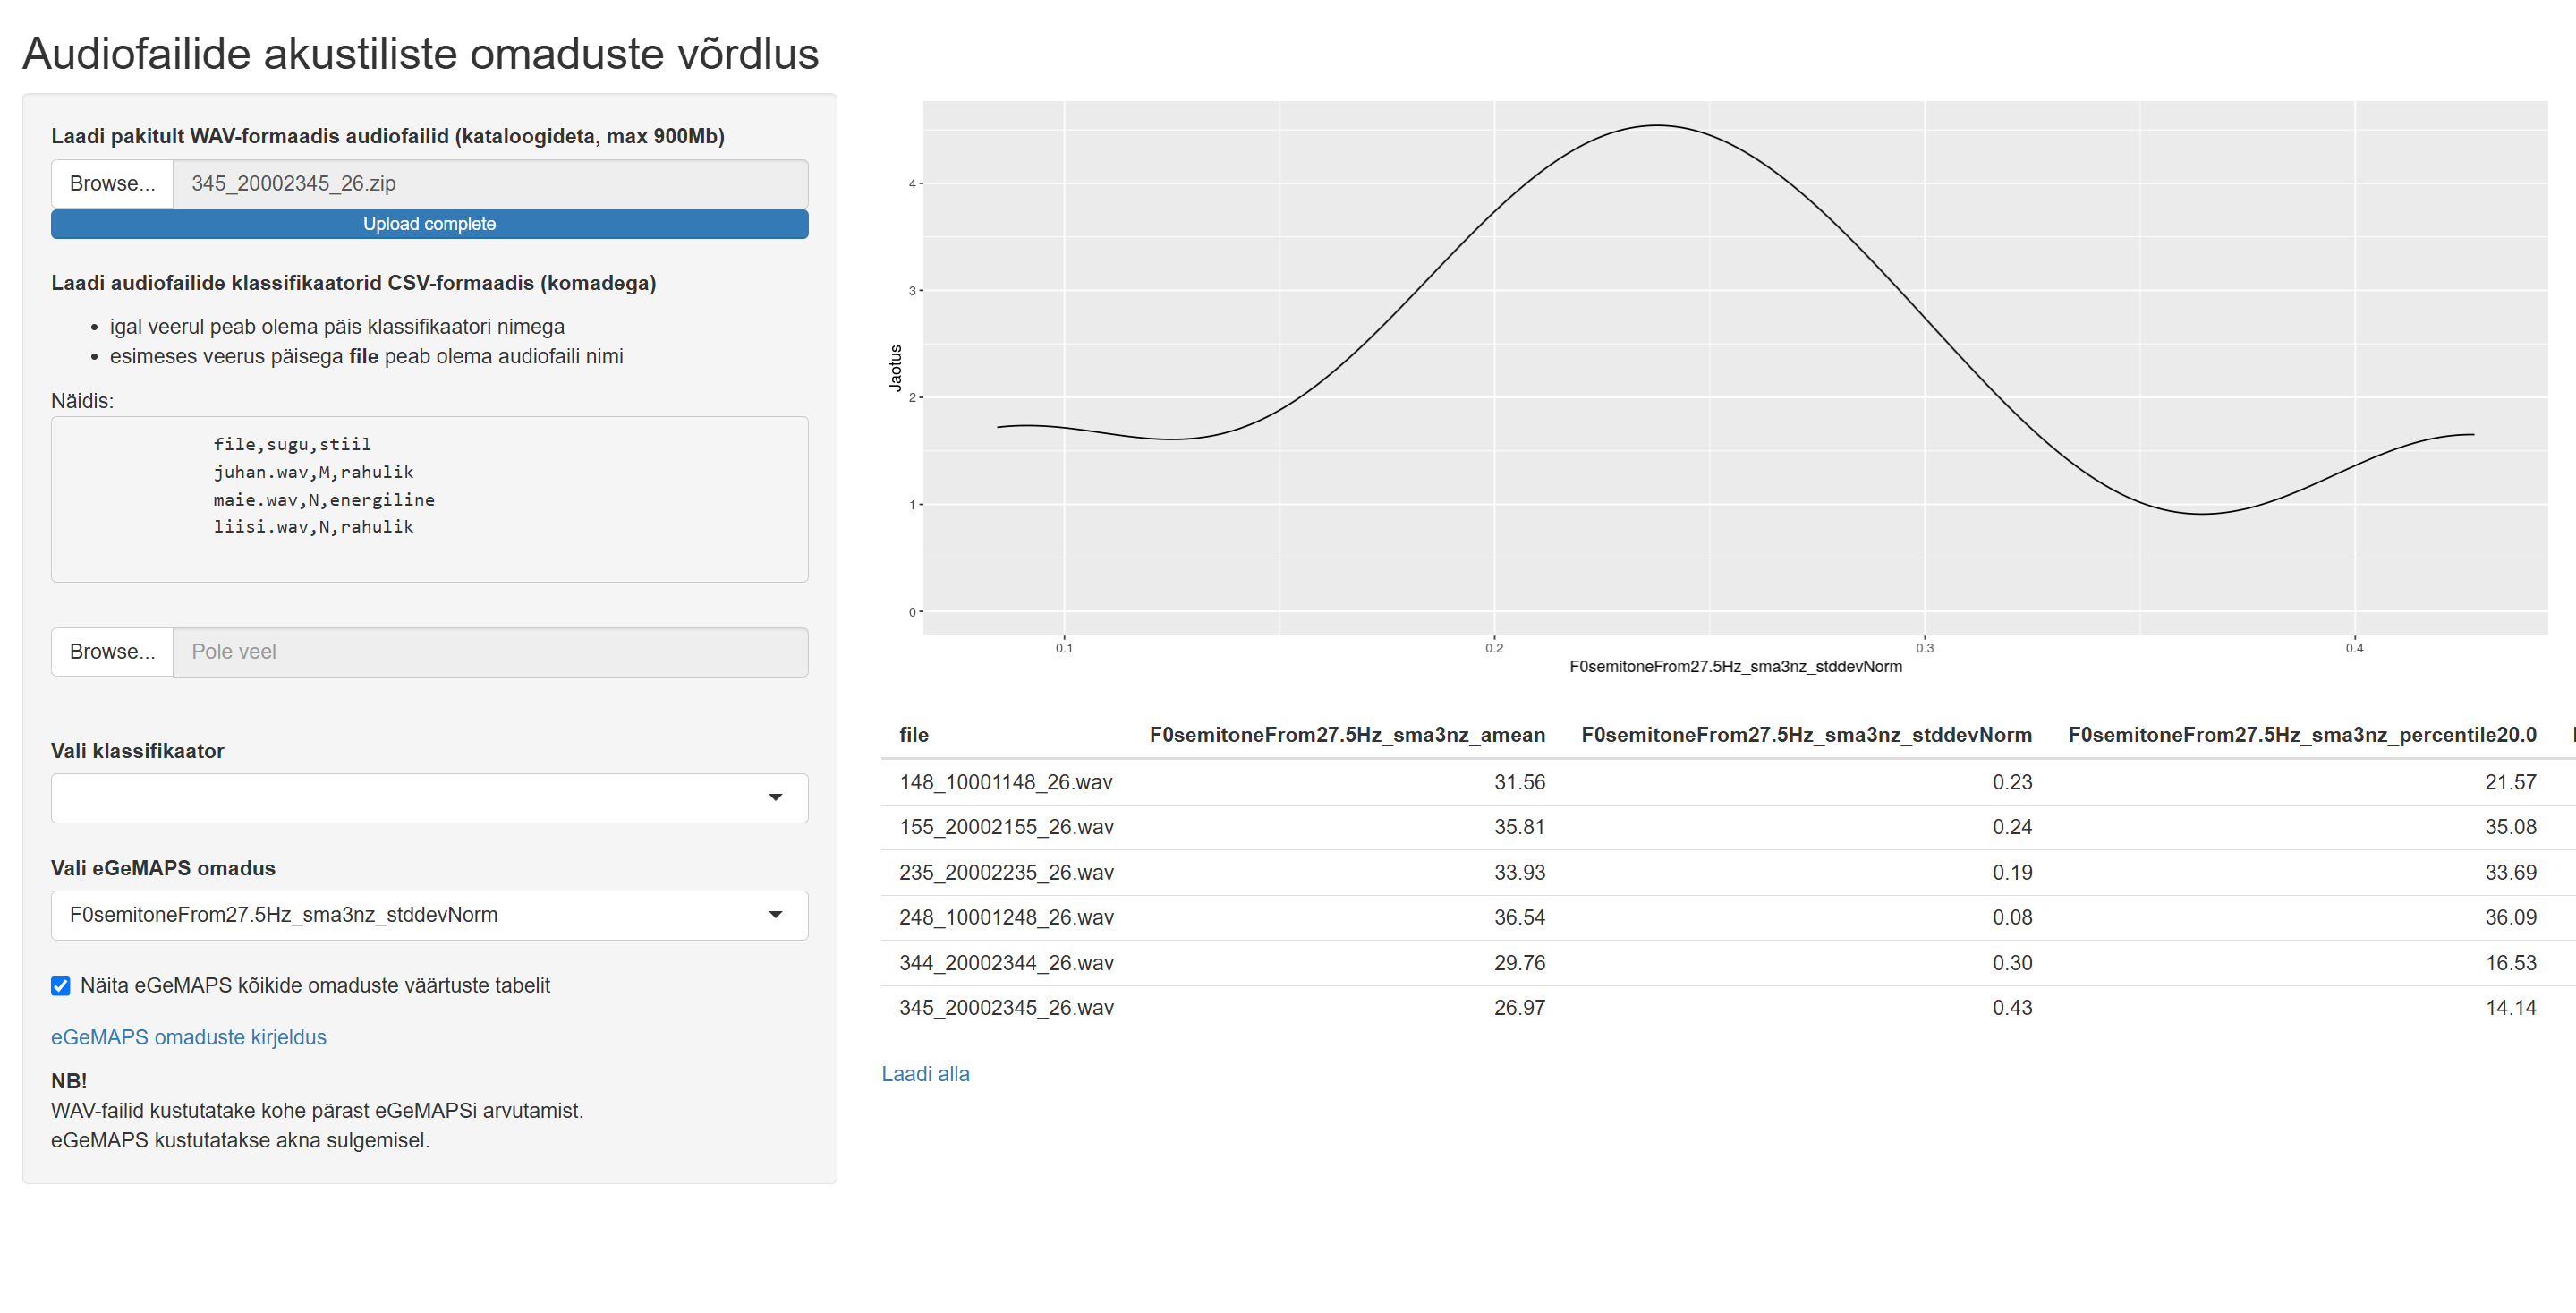
\includegraphics[width=\textwidth]{figures/alt-kõneveeb-põhivaade.png}
    \caption{\textit{Kõneveebi Audiofailide akustiliste omaduste võrdlemise rakenduse põhivaade}}
    \label{fig:alt-kõneveeb-põhivaade}
\end{figure}


\begin{longtable}{|p{2.5cm}|p{5.5cm}|p{5.5cm}|}
    \hline
    \textbf{Omadus} & \textbf{Kõneveeb} & \textbf{Loodud rakendus} \\
    \hline
    \endfirsthead
    \hline
    \textbf{Omadus} & \textbf{Kõneveeb} & \textbf{Loodud rakendus} \\
    \hline
    \endhead
    \hline
    \endfoot
    \hline
    \endlastfoot
    
    Tunnuste komplekt &
    Võimaldab analüüsida tervet 88 tunnusega eGeMAPS tunnustekomplekti. &
    Võimaldab analüüsida ainult eGeMAPS v02 LLD komplekti, mis sisaldab üksnes madala taseme deskriptoreid (LLD). \\
    \hline
    
    Rakenduse tüüp &
    Veebirakendus. &
    Installitav töölauarakendus, töötab lokaalselt. \\
    \hline
    
    Kasutajaliides &
    Sarnane põhivaate ülesehitusele nagu loodud rakendusel: kontrollpaneel valikutega vasakul ning paremal visualiseerimise ja andmetabeli sektsioonid. &
    Sarnane põhivaate ülesehitusele nagu kõneveebil: kontrollpaneel valikutega vasakul ning paremal visualiseerimise ja andmetabeli sektsioonid. \\
    \hline
    
    Erinevate graafikute valik &
    Joondiagramm. &
    Pakub laiemat valikut tunnuste graafikuid, sealhulgas ajatelje diagramm, histogramm, karpdiagramm, radardiagramm, vokaalikaart. Sarnasuse analüüsil on võimalik kasutada hajuv- ja tulpdiagramme. Samuti on graafikud interaktiivsed. \\
    \hline
    
    TexdGridide info kasutamine &
    Ei paku võimalust lugeda ega töödelda TextGrid-failides sisalduvaid ajaintervalle (sõnu, foneeme). Analüüs piirdub salvestuse tasemega. &
    Võimaldab lugeda TextGrid-faili, seostada konkreetsete tunnuste väärtusi sõna või foneemi ajaintervalliga ning seejärel kuvada eraldi vaateid/visualiseeringuid valitud segmentidele. \\
    \hline
    
    Sarnaste salvestuste leidmine &
    Puudub. &
    Võimaldab mitut sarnasuse arvutamise meetodit (klasterdamine, koosinussarnasus, PCA-järgne koosinussarnasus). Visualiseerib tulemused kas tulpdiagrammina (näiteks kõige sarnasemad salvestised) või hajuvdiagrammil, kus sihtsalvestis ja sarnased salvestised on esile tõstetud. \\
    \hline
    
    Andmete eksport &
    On nupp arvutatud tunnuste andmete allalaadimiseks, kuid see ei toiminud antud töö kirjutamise ajal. &
    Toetab andmete eksporti JSON faili ja pildifaili kujul. \\
    \hline
    
    Andmete haldus &
    Üleslaetud failid ja arvutatud tunnused kustutatakse seansi lõpus. Failide maht on piiratud (kuni 900 MB) ja tulemusi ei salvestata. &
    Kasutab MongoDB andmebaasi analüüsi andmete hoidmiseks. \\
    \hline

\end{longtable}

Kokkuvõttes on Kõneveebi rakendusel ja loodud rakendusel sarnane põhifookus, kuid veidi erinev ulatus. Kõneveeb on kindlasti mugav ja kiirem, kuna see ei vaja eraldi installeerimist ja seadistamist. Kuid käesolev rakendus on laiema funktsionaalsusega, terviklikum ning sobib paremini mahukamaks analüüsiks, kus on vaja erinevaid visualiseerimismeetodeid, analüüsitulemuste salvestamist ja sarnasuse analüüsi.

\section{Tagasiside}
Rakenduse valideerimiseks küsiti tagasisidet foneetikauurijalt. Uurijale saadeti rakenduse installeritav versioon, koos kasutusjuhendiga ja tagasisideküsimustega (Lisa. 2).

\section{Võimalused edasiarenduseks}
Rakendusel on palju võimalusi edasiarendusteks, näiteks:
\begin{itemize}
    \item Võimaldada erinevate tunnustekomplektide arvutamine
    \item Võimaldada erinevate normaliseerimismeetodite rakendamine/mitte rakendamine.
    \item Kasutajaliidese mugavdamine: näiteks menüüs võiks olla rohkem ruumi tunnuste ja salvestuste valimiseks
    \item Muuta rakendus veebirakenduseks
    \item Sarnasuse analüüsi valideerimine, rohkem meetodeid sarnaste salvestuste leidmiseks
    \item Andmete mahu probleemi lahendamine: kui andmete hulk kasvab, muutub rakendus aeglasemaks
\end{itemize}
